%%%%%%%%%%%%%%%%%%%%%%%%%%%%%%%%%%%%%%%%%%%%%%%
%%%     Declarations (skip to Begin Document, line 88, for parts you fill in)
%%%%%%%%%%%%%%%%%%%%%%%%%%%%%%%%%%%%%%%%%%%%%%%

%%\documentclass[10pt]{article}
%%\documentclass[10pt]{report}
%%\documentclass[letterpaper]{article}
\documentclass[12pt]{article}
\usepackage[hyperfootnotes=false]{hyperref}
\usepackage{geometry}
%\usepackage{xcolor}
\usepackage[table]{xcolor}
\usepackage{amsmath}
\usepackage[some]{background}
%\usepackage{lipsum}
%\usepackage{natbib}
\usepackage[utf8]{inputenc} % set input encoding to utf8

% V E R S I O N I N G
\usepackage{vhistory}

% U N I T S
%\usepackage[binary-units]{siunitx}
\usepackage[]{siunitx}

% L I N E  N U M B E R S
\usepackage{lineno}
%\linenumbers
 
% C I T A T I O N S
%\usepackage[backend=biber,style=apa]{biblatex}
\usepackage[backend=biber, style=apa, maxcitenames=1]{biblatex} 
%\DeclareLanguageMapping{english}{english-apa}
%\usepackage{apacite}
%\bibliographystyle{apa}

%\usepackage{biblatex} 
\addbibresource{paperpile.bib}
\usepackage{datetime}

%\usepackage{hyperref}

% Tables
\usepackage{float}
\usepackage[utf8]{inputenc}
\usepackage{tabularx}
\usepackage{booktabs}
\usepackage{longtable}

\usepackage{diagbox} %table split headers
\usepackage{longtable}
\usepackage{array}
\usepackage{rotating}
\usepackage{eqparbox}
\usepackage{makecell, caption, booktabs}
\usepackage{tablefootnote}

\usepackage{colortbl}

% Confusion Table
\usepackage{rotating}
\usepackage{xparse}
\usepackage{booktabs, makecell, multirow}
\NewExpandableDocumentCommand\mcc{O{1}m}
    {\multicolumn{#1}{c}{#2}}
\usepackage{siunitx}

% W A T E R M A R K 
% This gets rid of the draft watermark on the title page
\backgroundsetup{contents={}}
%\usepackage[text=DRAFT]{draftwatermark}

% L I N E  S P A C I N G
%\renewcommand{\baselinestretch}{1.5} 

% This does not have the effect I wanted, putting the caption at the bottom.
%\usepackage{caption}
%\captionsetup[table]{position=bottom} 

% Stuff needed to get table to span pages
\usepackage{enumitem}
%\usepackage{array, booktabs, longtable}
\newcolumntype{x}[1]{>{\raggedright}p{#1}}

\usepackage{etoolbox}
\AtBeginEnvironment{longtable}{%
    \setlist[itemize]{nosep,     % <-- new list setup
                      topsep     = 0pt       ,
                      partopsep  = 0pt       ,
                      leftmargin = *         ,
                      label      = $\bullet$ ,
                      before     = \vspace{-\baselineskip},
                      after      = \vspace{-0.5\baselineskip}
                        }
                           }% end of AtBeginEnvironment
% End table span

\definecolor{green}{rgb}{0.1,0.1,0.1}
%\color{green!40!yellow})

\newcommand{\done}{\cellcolor{teal}done}  %{0.9}
\newcommand{\hcyan}[1]{{\color{teal} #1}}

% Listings
\usepackage{listings}

\usepackage{geometry}  % Lots of layout options.  See http://en.wikibooks.org/wiki/LaTeX/Page_Layout
\geometry{letterpaper}  % ... or a4paper or a5paper or ... 
\usepackage{fullpage}  % somewhat standardized smaller margins (around an inch)
\usepackage{setspace}  % control line spacing in latex documents
\usepackage[parfill]{parskip}  % Activate to begin paragraphs with an empty line rather than an indent

\usepackage{amsmath,amssymb}  % latex math
\usepackage{empheq} % http://www.ctan.org/pkg/empheq
\usepackage{bm,upgreek}  % allows you to write bold greek letters (upper & lower case)

% for typsetting algorithm pseudocode see http://en.wikibooks.org/wiki/LaTeX/Algorithms_and_Pseudocode
\usepackage{algorithmic,algorithm}  

\usepackage{graphicx}  % inclusion of graphics; see: http://en.wikibooks.org/wiki/LaTeX/Importing_Graphics
% allow easy inclusion of .tif, .png graphics
\DeclareGraphicsRule{.tif}{png}{.png}{`convert #1 `dirname #1`/`basename #1 .tif`.png}

% \usepackage{subfigure}  % allows subfigures in figure
\usepackage{caption}
\usepackage{subcaption}

\usepackage{xspace}
\newcommand{\latex}{\LaTeX\xspace}

\usepackage{color}  % http://en.wikibooks.org/wiki/LaTeX/Colors

\long\def\todo#1{{\color{red}{\bf TODO: #1}}}

\long\def\ans#1{{\color{blue}{\em #1}}}
\long\def\ansnem#1{{\color{blue}#1}}
\long\def\boldred#1{{\color{red}{\bf #1}}}
\long\def\boldred#1{\textcolor{red}{\bf #1}}
\long\def\boldblue#1{\textcolor{blue}{\bf #1}}

% Useful package for syntax highlighting of specific code (such as python) -- see below
\usepackage{listings}  % http://en.wikibooks.org/wiki/LaTeX/Packages/Listings
\usepackage{textcomp}

% Table example start
\usepackage{booktabs, makecell}
\renewcommand\theadfont{\small\bfseries}
\usepackage{siunitx}
\usepackage{caption}

% Additional packages here
\usepackage{amsmath}
\usepackage{pdflscape}
% Table example end


%%% The following lines set up using the listings package
\renewcommand{\lstlistlistingname}{Code Listings}
\renewcommand{\lstlistingname}{Code Listing}

%%% Specific for python listings
\definecolor{gray}{gray}{0.5}
\definecolor{green}{rgb}{0,0.5,0}

\lstnewenvironment{python}[1][]{
\lstset{
language=python,
basicstyle=\footnotesize,  % could also use this -- a little larger \ttfamily\small\setstretch{1},
stringstyle=\color{red},
showstringspaces=false,
alsoletter={1234567890},
otherkeywords={\ , \}, \{},
keywordstyle=\color{blue},
emph={access,and,break,class,continue,def,del,elif ,else,%
except,exec,finally,for,from,global,if,import,in,i s,%
lambda,not,or,pass,print,raise,return,try,while},
emphstyle=\color{black}\bfseries,
emph={[2]True, False, None, self},
emphstyle=[2]\color{green},
emph={[3]from, import, as},
emphstyle=[3]\color{blue},
upquote=true,
morecomment=[s]{"""}{"""},
commentstyle=\color{gray}\slshape,
emph={[4]1, 2, 3, 4, 5, 6, 7, 8, 9, 0},
emphstyle=[4]\color{blue},
literate=*{:}{{\textcolor{blue}:}}{1}%
{=}{{\textcolor{blue}=}}{1}%
{-}{{\textcolor{blue}-}}{1}%
{+}{{\textcolor{blue}+}}{1}%
{*}{{\textcolor{blue}*}}{1}%
{!}{{\textcolor{blue}!}}{1}%
{(}{{\textcolor{blue}(}}{1}%
{)}{{\textcolor{blue})}}{1}%
{[}{{\textcolor{blue}[}}{1}%
{]}{{\textcolor{blue}]}}{1}%
{<}{{\textcolor{blue}<}}{1}%
{>}{{\textcolor{blue}>}}{1},%
%framexleftmargin=1mm, framextopmargin=1mm, frame=shadowbox, rulesepcolor=\color{blue},#1
framexleftmargin=1mm, framextopmargin=1mm, frame=single,#1
}}{}
%%% End python code listing definitions

\DeclareMathOperator{\diag}{diag}
\DeclareMathOperator{\cov}{cov}


%\bibliography{./paperpile.bib}
%\author{Evan McGinnis}
%\title{Automated Weeding}



\definecolor{titlepagecolor}{cmyk}{1,.60,0,.40}

\DeclareFixedFont{\bigsf}{T1}{phv}{b}{n}{1.5cm}

\backgroundsetup{
scale=1,
angle=0,
opacity=1,
contents={\begin{tikzpicture}[remember picture,overlay]
 \path [fill=titlepagecolor] (-0.5\paperwidth,5) rectangle (0.5\paperwidth,10);  
\end{tikzpicture}}
}
\makeatletter                       
\def\printauthor{%                  
    {\large \@author}}              
\makeatother
\author{%
\setstretch{1.0}
    Evan McGinnis \\
    PhD Student \\
    Student ID\#  23633780\\
    Biosystems Analytics \\
    \today \\
    \texttt{evanmc@arizona.edu}\vspace{40pt} \\
    }

\begin{document}

\begin{titlepage}
\BgThispage
\newgeometry{left=1cm,right=4cm}
\vspace*{1cm}
\noindent
%%\vspace*{0.4\textheight}
\textcolor{white}{\Huge\textbf{\textsf{Proposal for the Study of Weed/Crop\\Discrimination in Row Crops}}}
\vspace*{2.5cm}\par
\noindent
\begin{minipage}{0.35\linewidth}
    \begin{flushright}
        \printauthor
    \end{flushright}
\end{minipage} \hspace{15pt}
%
\begin{minipage}{0.02\linewidth}
    \rule{1pt}{175pt}
\end{minipage} \hspace{-10pt}
%
\begin{minipage}{0.8\linewidth}
\vspace{5pt}
    \begin{abstract} 
\setstretch{1.0}
This paper proposes a study of classification of vegetation as weeds and crop of plants found within a spinach field at various heights AGL, and how those classifications can be used to produce high-precision treatment plans. This study will examine the classification of visible-light images acquired from unmanned aerial vehicle flights at various altitudes ranging from 3 to 30 meters. Specifically, the first phase will produce the optimal set of attributes for classification using seven different Machine Learning techniques at each altitude. The second phase will concentrate on the production of treatment plans from those classifications.  While this phase will produce treatment plans that can be explored with an application developed as part of this phase or executed by human referencing a summary (PDF) of the plan, extending these plans to automated treatment does not require substantial changes. The execution of a treatment plan is not explicitly addressed by this study, but the framework developed as part of this study will support a near realtime treatment application system.
    \end{abstract}
\end{minipage}
\end{titlepage}
\restoregeometry
%
% F R O N T  M A T T E R
%
{
\setstretch{1.0}
\tableofcontents
\listoftables
\listoffigures
\newpage
}

{
\setstretch{1.0}
\begin{versionhistory}
  \vhEntry{1.0}{1 Aug 2023}{EM}{Initial revision}
  \vhEntry{1.1}{7 Aug 2023}{EM}{Incorporate comments}
  \vhEntry{1.1}{30 Nov 2023}{EM}{Incorporate comments and remove lettuce references. Revise introduction and add section on color correction.}
\end{versionhistory}
\newpage
}


%
% O V E R V I E W
%

\section{Overview}
\label{section:proposal}
The classification of vegetation found with an image into two classes (desired and undesired) is essential to whatever sort of precision treatment is planned, whether that treatment is the elimination of undesired vegetation through chemical or mechanical means or the enhancement of desired vegetation through the application of synthetic fertilizer. Manual weed control by mechanical means in row crops is expensive, and labor willing to perform this field work is increasingly hard to find. Alternatively, weed control (as well as crop enhancement) using manual chemical application is not only expensive, but is a harm to both the environment and worker's health.  This study will produce a set of approaches and parameters that can be used at various distances to ensure accurate classification as a first step toward subsequent treatment using a much smaller volume of harmful chemicals than would be used in manual application or more effective manual weed control.

 While it is tempting to use the terms \textit{weed} and \textit{crop} (and this document will often use those terms), this proposal will more often reference vegetation as \textit{desired} (crop in the position wanted) and \textit{undesired} (weeds and crop not in the position wanted).  That is, classification more often answers the question ``do we want this plant'' than ``is this plant a weed''. These two questions are often conflated, but are subtly distinct.

 Images from UAVs offer several advantages over those obtained with manned aircraft and satellite, such as the economics or flexibility of acquisition, but this study will leverage the relative ease with which UAVs are able to gather imagery from various distances close to the ground. While many studies use images gathered close to the ground from a single distance and report classification accuracy and others use images gathered at multiple distances, reporting (the inevitably declining) accuracy seen with increasing distance, the former tends to suffer when the same attributes are applied at higher distances and the latter from holding the set of attributes constant as altitudes increase. \citeauthor{Ong2023-lm}, in a study of classification of Chinese Cabbage, classifies vegetation acquired at an average of 2m AGL using a single set of attributes, Local Binary Pattern (LBP, a texture descriptor), and a single approach (Random Forest) leveraging those attributes, validating the use of texture in classification \parencite{Ong2023-lm}. \citeauthor{Etienne2021-ik}, in a study of Corn and Soybean plots, used imagery gathered from both 10m and 30m AGL. but found that the best training set for selected algorithm (YOLOv3) was taken from the set of images acquired from 10m \parencite{Etienne2021-ik}. The parameters selected as significant to classification fall into three basic categories: shape, color, and texture. Variants of each of these categories will be used in this study. 
In a study of weed mapping in sunflower crop, \citeauthor{Perez-Ortiz2015-yk} present findings from images taken from three distances AGL, 30m, 60m, and 100m, classifying each pixel as crop, weed, or soil using SVM, KNN, and k-means (and variants of those) approaches \parencite{Perez-Ortiz2015-yk}. While this approach does indeed yield weed maps that lend themselves to later study, the approach is a bit different in terms of what is being classified. In that study, individual pixels are being classified, in contrast to this study that seeks to classify individual plants.
In a study of weeds in corn, \citeauthor{Lin2017-xq} used shape metrics as part of the classification workflow, stressing the importance of expressing shape metrics that are not rotationally variant. More importantly, the study details a shape metric possessing the desired qualities for use in classification. Using shape and texture (GLCM), the study demonstrated an overall accuracy exceeding 95\%.\footnote{\citeauthor{Lin2017-xq}'s study did not report some items that are of interest: the distances of the imagery to the camera, and the false positive rate of weed identification. While the high overall rate sounds is certainly impressive, that metric will not be used in this study. Additionally, the images of vegetation were acquired under controlled conditions, something that is not reproducible in the field an at higher distances AGL.} \citeauthor{Sabzi2020-af}, in a study of a potato field, used various channels of color spaces (YIQ, YCbCr, HSI) as well as texture (Grey-Level Co-occurrence Matrix, GLCM) to achieve a high correct classification rate, but the use of GLCM is not applied  to channels of the color conversion, only to RGB images that have been converted to greyscale \parencite{Sabzi2020-af}. While this is a conventional use of the texture identification technique, it does not leverage the information content available in other color spaces.

This study will take a different approach, and will produce sets of optimal parameters extracted from visible light images for various machine learning (ML) techniques acquired from various distances AGL in the first phase and will support the exploration of those classifications through a tablet-based application and the production of treatment plans in the second. The parameters extracted for each plant include various color, shape, and textural attributes. The classification approaches will use labeled data and include Random Forest, Logistic Regression, KNN, Decision Tree, Support Vector Machine, and Linear Discriminate Analysis. Features that may be significant at a low altitude (the shape of leaves, for example) may not be as significant at higher altitudes (as the shape of all leaves may tend to be much the same). That is, at the conclusion of this study, the analysis will produce something along the lines of Table~\ref{tab:example}, where techniques and parameter extraction can be determined by flight altitude.\footnote{This table is, of course, is just an example with no basis in reality. The final table produced will also include a data on what is to be accomplished: eliminate weeds or enhance crop. While much of the literature and studies concentrate on detecting weeds, doing so is sometimes not the overriding concern if the treatment is to enhance the crop. Accurate detection of the latter is more important than the former.} This will fill a void identified in current research, specifically: \textit{If I fly a drone at distance X AGL, what parameters should I use to get the best result for a given treatment?}. While this study will produce other outputs, these findings will be the most directly useful.
 \begin{table}[h]
	\centering
    \caption{Example parameters at AGL}
    \label{tab:example}
    \begin{tabular}[t]{lll} 
		\textbf{AGL} & \textbf{Classification Technique} &\textbf{Parameters}\\
		\midrule
			3 & Logistic Regression & Shape, GLCM (Texture)\\
			5 & Logistic Regression & GLCM, HOG\\
			10 & Support Vector & GLCM, HOG\\
			15 & Support Vector & GLCM, Color\\
			30 & Random Forest & GLCM, Color\\
    \end{tabular}
\end{table}

 The scoring of the ML models will not be through examining overall accuracy, but by considering the treatment to be applied.  For a negative treatment (one in which plants are eliminated) employing a cost-based model where the misclassification of a crop as a weed is more costly than misclassification of a weed as crop is applicable. While weeds that remain after a classification and treatment will continue to consume resources and compete with crop, creating indirect costs, the misclassification and subsequent treatment of a crop plant has direct cost. That is, mistaking a weed for a crop (here, a false positive), while bad, is not nearly as bad as mistaking a crop for a weed (here, a false negative). Likewise, the opposite would hold true for positive treatments -- enhancing the health of a weed is not a desirable use of resources.  Many of the studies cited in this introduction used Principal Components Analysis (PCA) as the method to identify significant parameters. And while PCA will be one of the techniques used in parameter identification, this study will also use other techniques, as early findings have shown that while using parameters identified with PCA may yield acceptable results for some ML techniques, using those same parameters for others often yields poor results. Using parameters discovered with a different technique (Recursive Elimination, perhaps) corrects this poor performance, using the same data.
 
 The discovery of the optimal set at each altitude will involve the University of Arizona's High Performance Compute Cluster to build and assess models built with the most significant subset of parameters extracted for all techniques mentioned.
 
While exposing it is not a direct output of this study, this word will also produce a labeled dataset hosted within a database that can be used in subsequent work. This dataset is supported by utility scripts and an API that allows production of datasets for a given crop, distance AGL, location, or time. Use of databases may be present in the studies examined for this proposal, but those studies offered, at best, ``data used in this study is available on request''. Consequently, it is difficult to say with any certainty how the data is managed. 
 
 The second phase of this project will explore the production of treatment plans from classifications. Treatment plans can be explored by a user with an application, summarized into reports (PDF), and used in automated treatment systems.  While the second phase of this proposal will  produce plans that are focused on the first two, the infrastructure and classifications provided by the system will allow for further development in this area.

\section{Location and Subject of Study}
This study will be carried out at the University of Arizona Maricopa Agricultural Center (MAC) on a spinach crop overseen by Drs. Attalah and Elshikha (University of Arizona), as part of another study.\footnote{The field in question is located at N 33.061805$^{\circ}$ W 111.966162$^{\circ}$} That study will involve three separate water treatments: center-pivot, flood irrigation, and drip. As the drip treatment study area is unlikely to produce a heavy weed load, it will not be included in this study, as differentiating between crop and weeds is an initial goal of this study. The planting date for the field is anticipated to be early December 2023, with image collection beginning mid-January 2024. The study site is relatively free of obstacles that would impact low level flight with one notable exception: the center pivot irrigation system. Allowances will be made to avoid that system, but doing so is not expected to affect flight plans, as images in only subset of the field is planned to be captured.
 
\section{Phase I}
Phase I of this study will produce a prediction model for weeds that will exceed 80\% correct classification at altitudes of 10m AGL and lower, but will find the set of attributes and technique that can be applied at various heights AGL between 3m and 30m. The model produced in this phase can be applied for fields with the same crop, regardless of when in the development cycle those predictions are made. 


\subsection{Workflow}
The workflow shown in Figure~\ref{fig:workflow-image} indicates the operations performed on each image, the details of which will be discussed in subsequent sections.  The workflow consumes the images acquired in the field, processes them, and places them in a database.  While the processing of data and the extraction of features is carried out off-line, those operations can be accomplished in a sub-second time frame. While images originally obtained in the field can be retained after processing, doing so is not required, as the two subsequent operations reference items within the database: labeling the dataset, and classification using the extracted features. The step shown in the image processing workflow as \textit{Label Blobs} takes much longer, of course, as a human uses an application to indicate if a plant is a weed or a crop. 
\begin{figure}[h!]
	\centering
	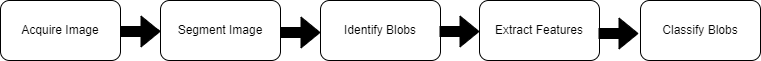
\includegraphics[width=0.8\linewidth]{./figures/workflow.drawio.png}
	\caption[Image Workflow]{The image processing workflow results in each image broken down into individual plants within the image, and then the manual labeling of each one of those plants. This workflow does not explicitly show the use of the features extracted and placed in the database to classify each plant found, but this workflow shows the processing steps involved with each set of images to build that database.}
	\label{fig:workflow-image}
\end{figure}


\subsection{Image Acquisition}
\label{sec:acquisition}
Image acquisition will be the only activity taking place in the field; all other activities are conducted within the context of an office or datacenter. Images will be acquired from two sources: manually via hand-held camera for distances below one meter AGL, and automatically via planned missions for a UAV for distances between 2 and 30 meters AGL.\footnote{While admittedly arbitrary, this will allow inclusion of image acquisition where extremely-low altitude flights of AUV may present too much risk to merit inclusion. The intent of manual acquisition is to approximate the perspective seen in tractor-towed solutions, where the camera is much closer to the ground. If the risk of having a UAV fly at a low altitude is acceptable, manual acquisition is not required. Large portions of the field in this study are free of obstacles, allowing for low-risk, low distance AGL flights.} In both cases, only a subset of the study field will be captured. Image sets are acquired every two weeks during the crop development cycle and altitudes of 1m, 2m 5m, 10m, 15m, 20m, 25m, and 30m. Capturing images at varying altitudes is needed here to study the effects of feature significance with increased distance.
UAV images will be obtained with a DJI Mavic Air 2S equipped with a 256GB flash drive and using its stock 20MP visible-light camera.\footnote{Not included in this proposal is the prospect of gathering multispectral data via the UAV. While this proposal discusses the processing of visible wavelengths of light, nothing precludes including that data.} Each image set acquisition will be preceded by the imaging of a color calibration target.  While it may be an end goal of this study to produce a system that is not affected by changes in lighting conditions brought on by time of day or ambient conditions affected by cloud cover, acquisition of a color plate image will allow color corrected images to be used. Figure \ref{fig:mission} illustrates a image acquisition mission at 3 meters AGL, capturing an area of approximately 0.5 ha.

\begin{figure}[h!]
	\centering
	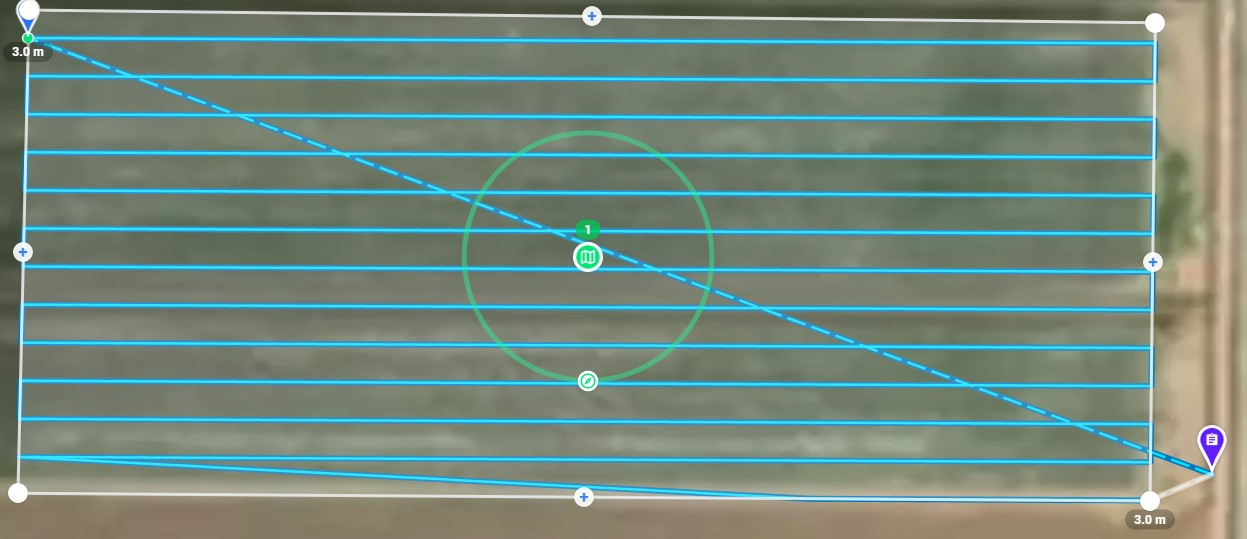
\includegraphics[width=0.8\linewidth]{./figures/maricopa-drone-3m.jpg}
	\caption[Semple UAV mission]{Sample UAV mission conducted at 3 meters capturing an area of approximately 0.5 ha. While this flight and capture orientation is not essential, this same mission plan will simply be repeated at higher altitudes.}
	\label{fig:mission}
\end{figure}

Table \ref{tab:acquisition} provides a summary of some attributes relevant to the image capture at various distances AGL.  Of special note here is the battery requirements, which are noted in the number of batteries required to complete the mission at that particular distance AGL. While a lower altitude flight will likely require two batteries to complete to allow for a wide safety margin, the remaining flights can be completed on the same battery.\footnote{Power consumption from the UAV is dependent, of course on conditions such as wind, so times and battery requirements are not exact projections}
The UAV has been equipped with a 256GB flash and has 8GB of internal storage. This total capacity far exceeds the projected storage requirements of even uncompressed images.\footnote{Digital Negatives (DNG), often referred to as \textit{raw images} is uncompressed sensor data. This sensor data can, of course, be converted to a much smaller, compressed format such as JPG, but can be more readily processed for color and exposure by programs such as Adobe Lightroom or Photoshop. It is a reasonable simplification to think of the storage requirements as a worst case scenario, as the storage of a less flexible, but smaller, format such as JPG, would allow for storage of significantly more images.  As an example, a DNG on the UAV selected would require around 24.5 MB, while an equivalent JPG would require 6.5 MB. Using the raw sensor data as part of the image processing workflow will have no impact on image quality -- in fact, converting raw sensor data to JPG is precisely what the UAV is doing. Retaining raw sensor data and then converting achieves the same goal.}
\begin{table}[ht]
	\centering
    \caption{Image Acquisition Mission Characteristics}
    \label{tab:acquisition}
    \begin{tabular}[t]{llllll} 
		\textbf{AGL} & \textbf{Photos} &\textbf{Storage (GB)} & \textbf{Time} & \textbf{Batteries} & \textbf{GSD (cm)}\\
		\midrule
		      3 & 554 & 13.6 & 20.37 & 2 & 0.06 \\
		      10 & 42 & 1.0  & 2:50 & 1 & 0.14 \\
		     15 & 18 & 0.4 & 2:17 & 1 & 0.28 \\
		     20 & 7 & 0.2 & 1:30 & 1 & 0.43 \\
		     25 & 6 & 0.1 & 1:30 &1 & 0.57 \\
		     30 & 5 & 0.1 & 1:30 & 1 & 0.71
    \end{tabular}
\end{table}

Of special note here is the GSD captured by a single pixel within an image and the relationship to the features extracted.  In early stages of development vegetation may be only a few square cm in size. A 25 cm$^2$ plant would be represented by 35 pixels. This low pixel representation is expected to negatively affect classification using color attributes. As \citeauthor{Iqbal2021-yx} state in a study of classification of four different crops, early crops are so similar in color that textural attributes are more effective. Shape attributes are expected to be ineffective for classification at this stage, as fine details of the shapes of both weeds and crop are not present in this resolution.

\subsection{Image Correction}
The images in different sets of the same area acquired suffer from two problems: they are acquired under uncontrolled conditions, and the conversion to readily consumed formats like JPG tend to be the camera system's best approximation of what the actual colors in the scene are. While an attempt will be made to collect images under roughly identical circumstances will be made to address the first problem, ambient lighting condition changes introduced by environmental conditions such as cloud cover make it unrealistic to completely match lighting from one collection to the next. In an attempt to match the colors from capture set to capture set, the workflow will first color-correct the images before subsequent processing is performed. While this will not compensate for the change in lighting conditions (consider how `bright' an image is), but will result in image sets where colors are matched where they would otherwise be distorted by the ambient light. This is particularly important for multiple camera systems -- the color rendition of an iPhone's camera, for instance, is unlikely to match that from the camera on a DJI drone. Each image acquisition will be preceded by a capture of a color correction target for use in this step, and commercially available software will be used to correct each image. As the color of an object is slated to be a factor used in classification, accurate color rendition supports this objective.

\subsection{Image Segmentation and Blob Identification}
The details of the image segmentation techniques will be covered in-depth in a separate document, but several approaches will be evaluated to separate vegetated and non-vegetated pixels, including CIVE, Excess Green, Excess Red, NGRDI, Vegetative Index, and Triangular Greenness Index \parencite{Hunt2013-ih,Hamuda2016-dw}. These indices are used to create a mask that is then applied to the original source image to permit vegetation to show while masking details that are not relevant (ground pixels, stones, and other items that may appear in field conditions) The intent here is to remove all pixels that are not relevant to the task of distinguishing between crop and weed while leaving the vegetated pixels unmanipulated. At this, as with all steps, computational efficiency will be evaluated, as it is the goal to have the system operate in real-time.
\begin{figure}[H]
	\centering
	\begin{subfigure}[h]{.20\textwidth}
	  \centering
	  \includegraphics[width=1\linewidth]{figures/original.jpg}
	  \caption{Field view}
	  \label{fig:original}
	\end{subfigure}
	\begin{subfigure}[h]{.20\textwidth}
	  \centering
	  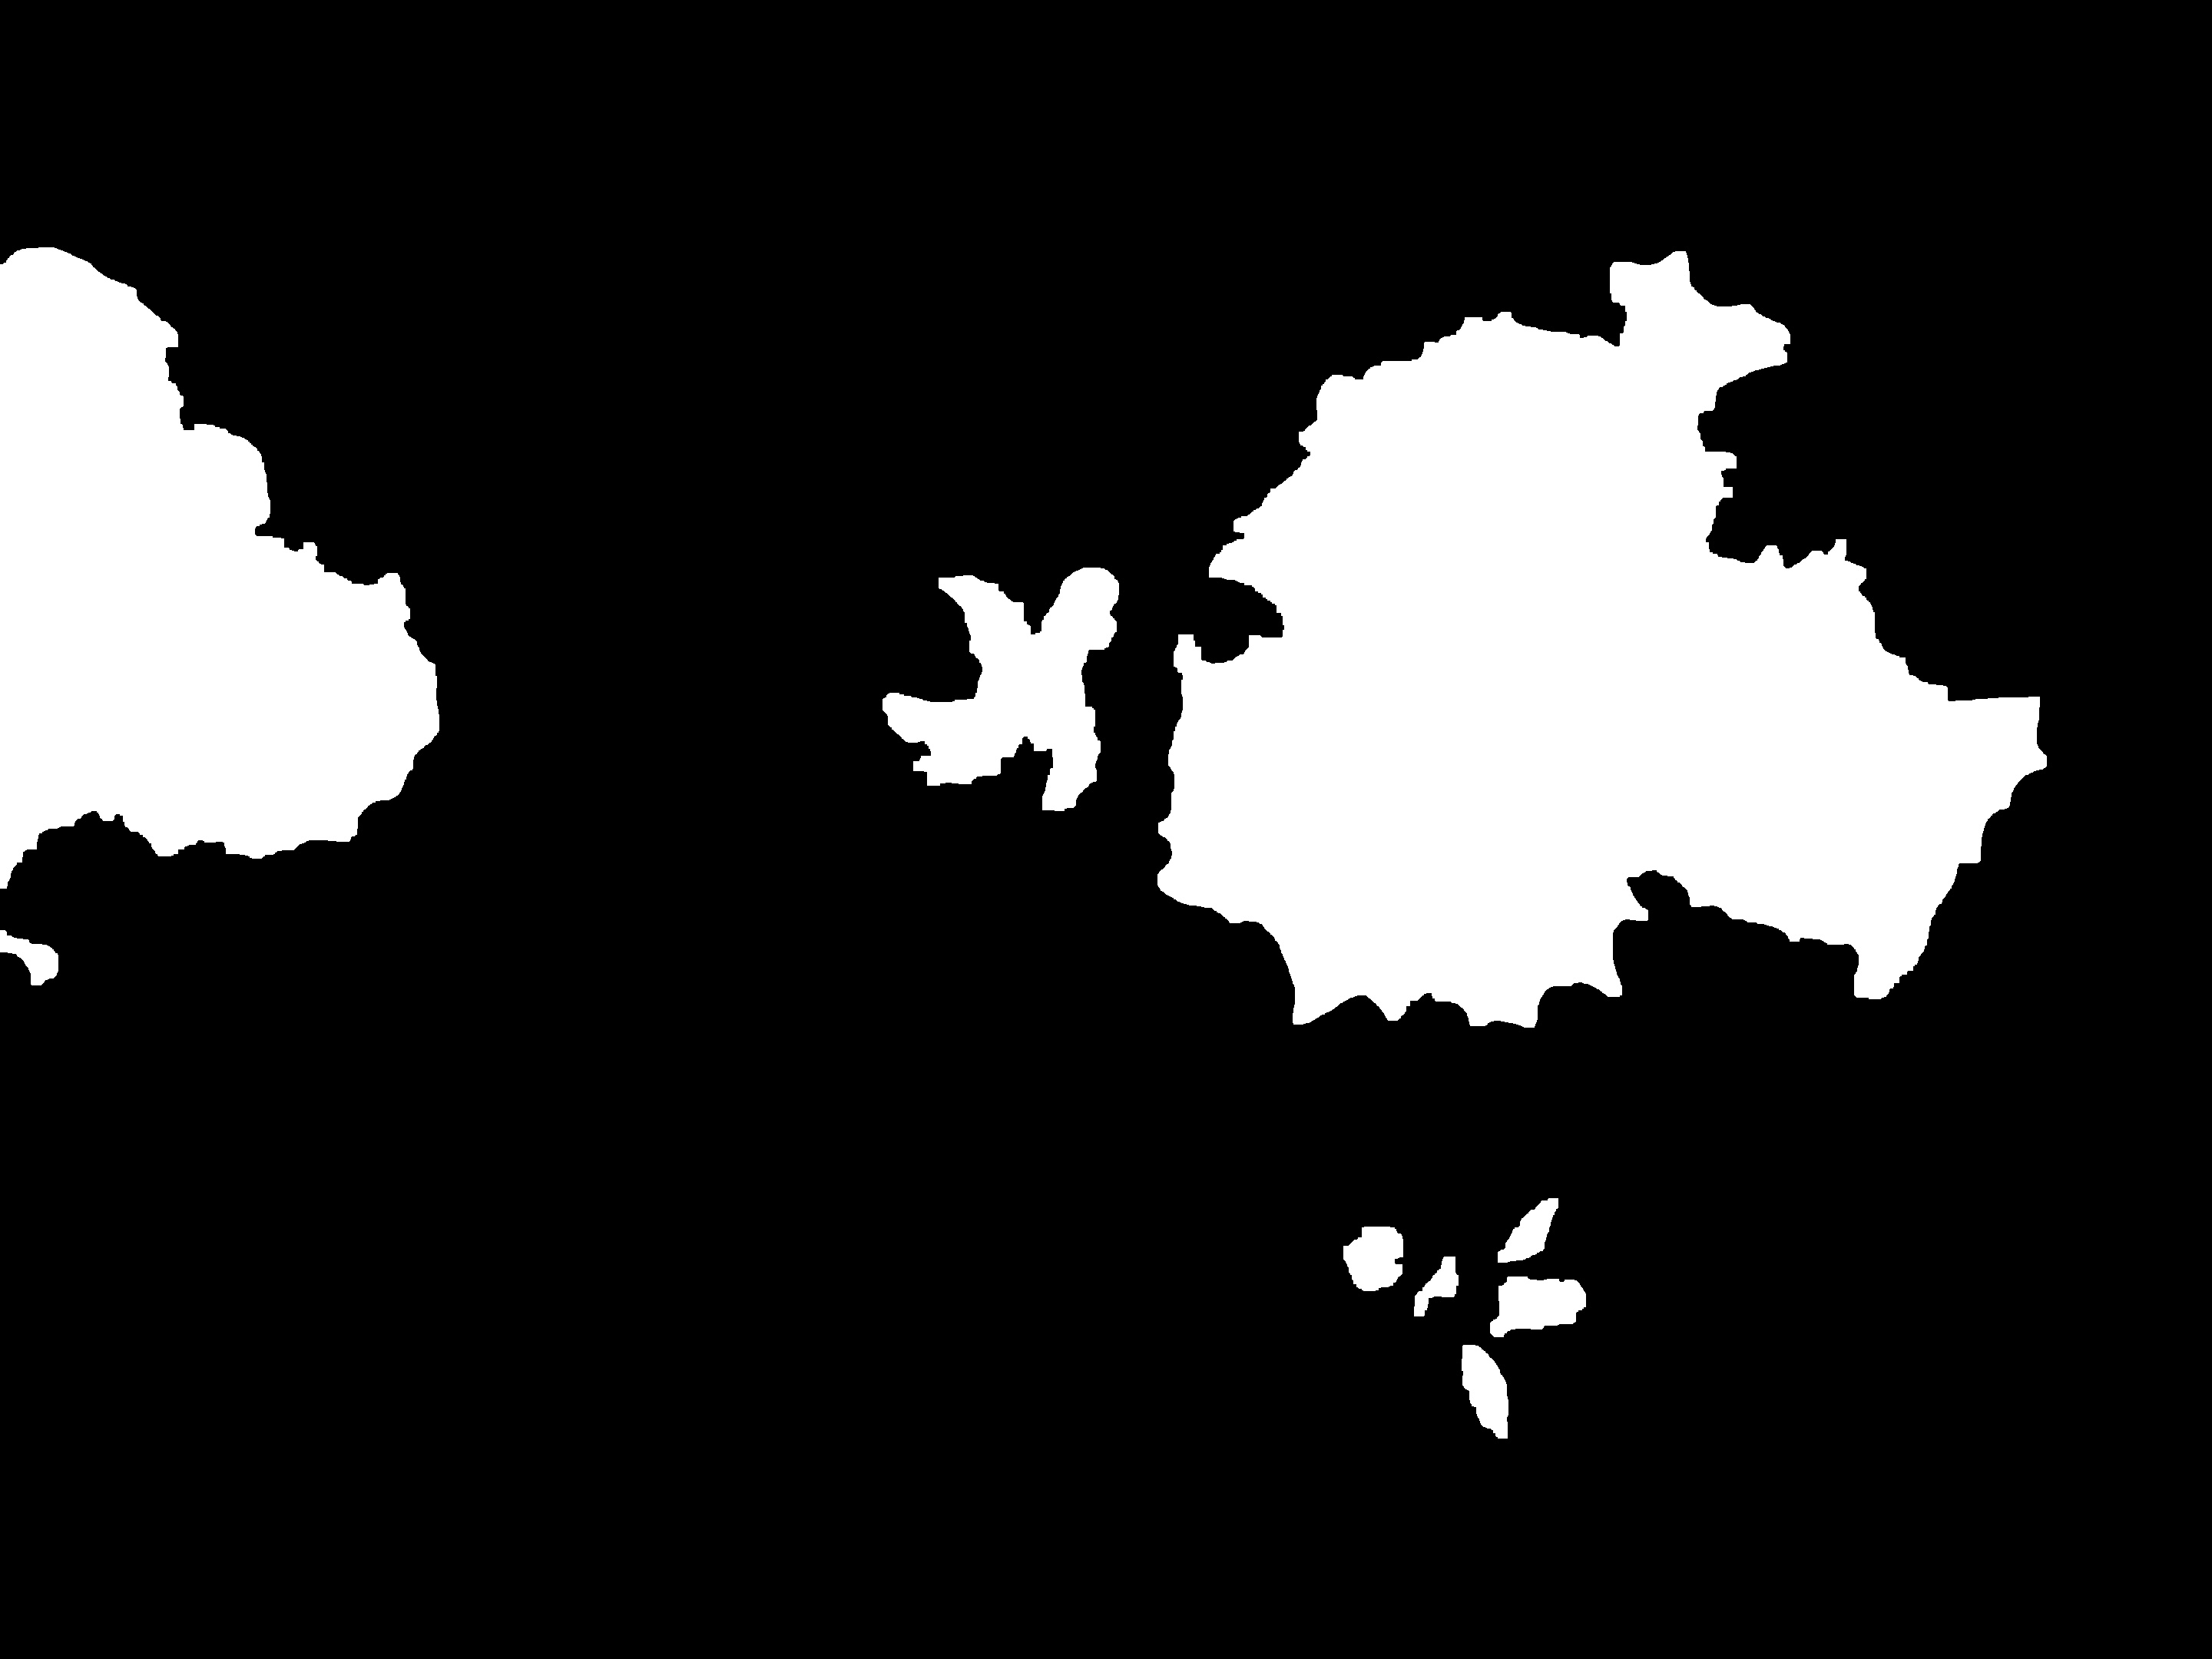
\includegraphics[width=1\linewidth]{figures/original-mask.jpg}
	  \caption{NDI mask}
	  \label{fig:mask}
	\end{subfigure}
	\begin{subfigure}[h]{.20\textwidth}
	  \centering
	  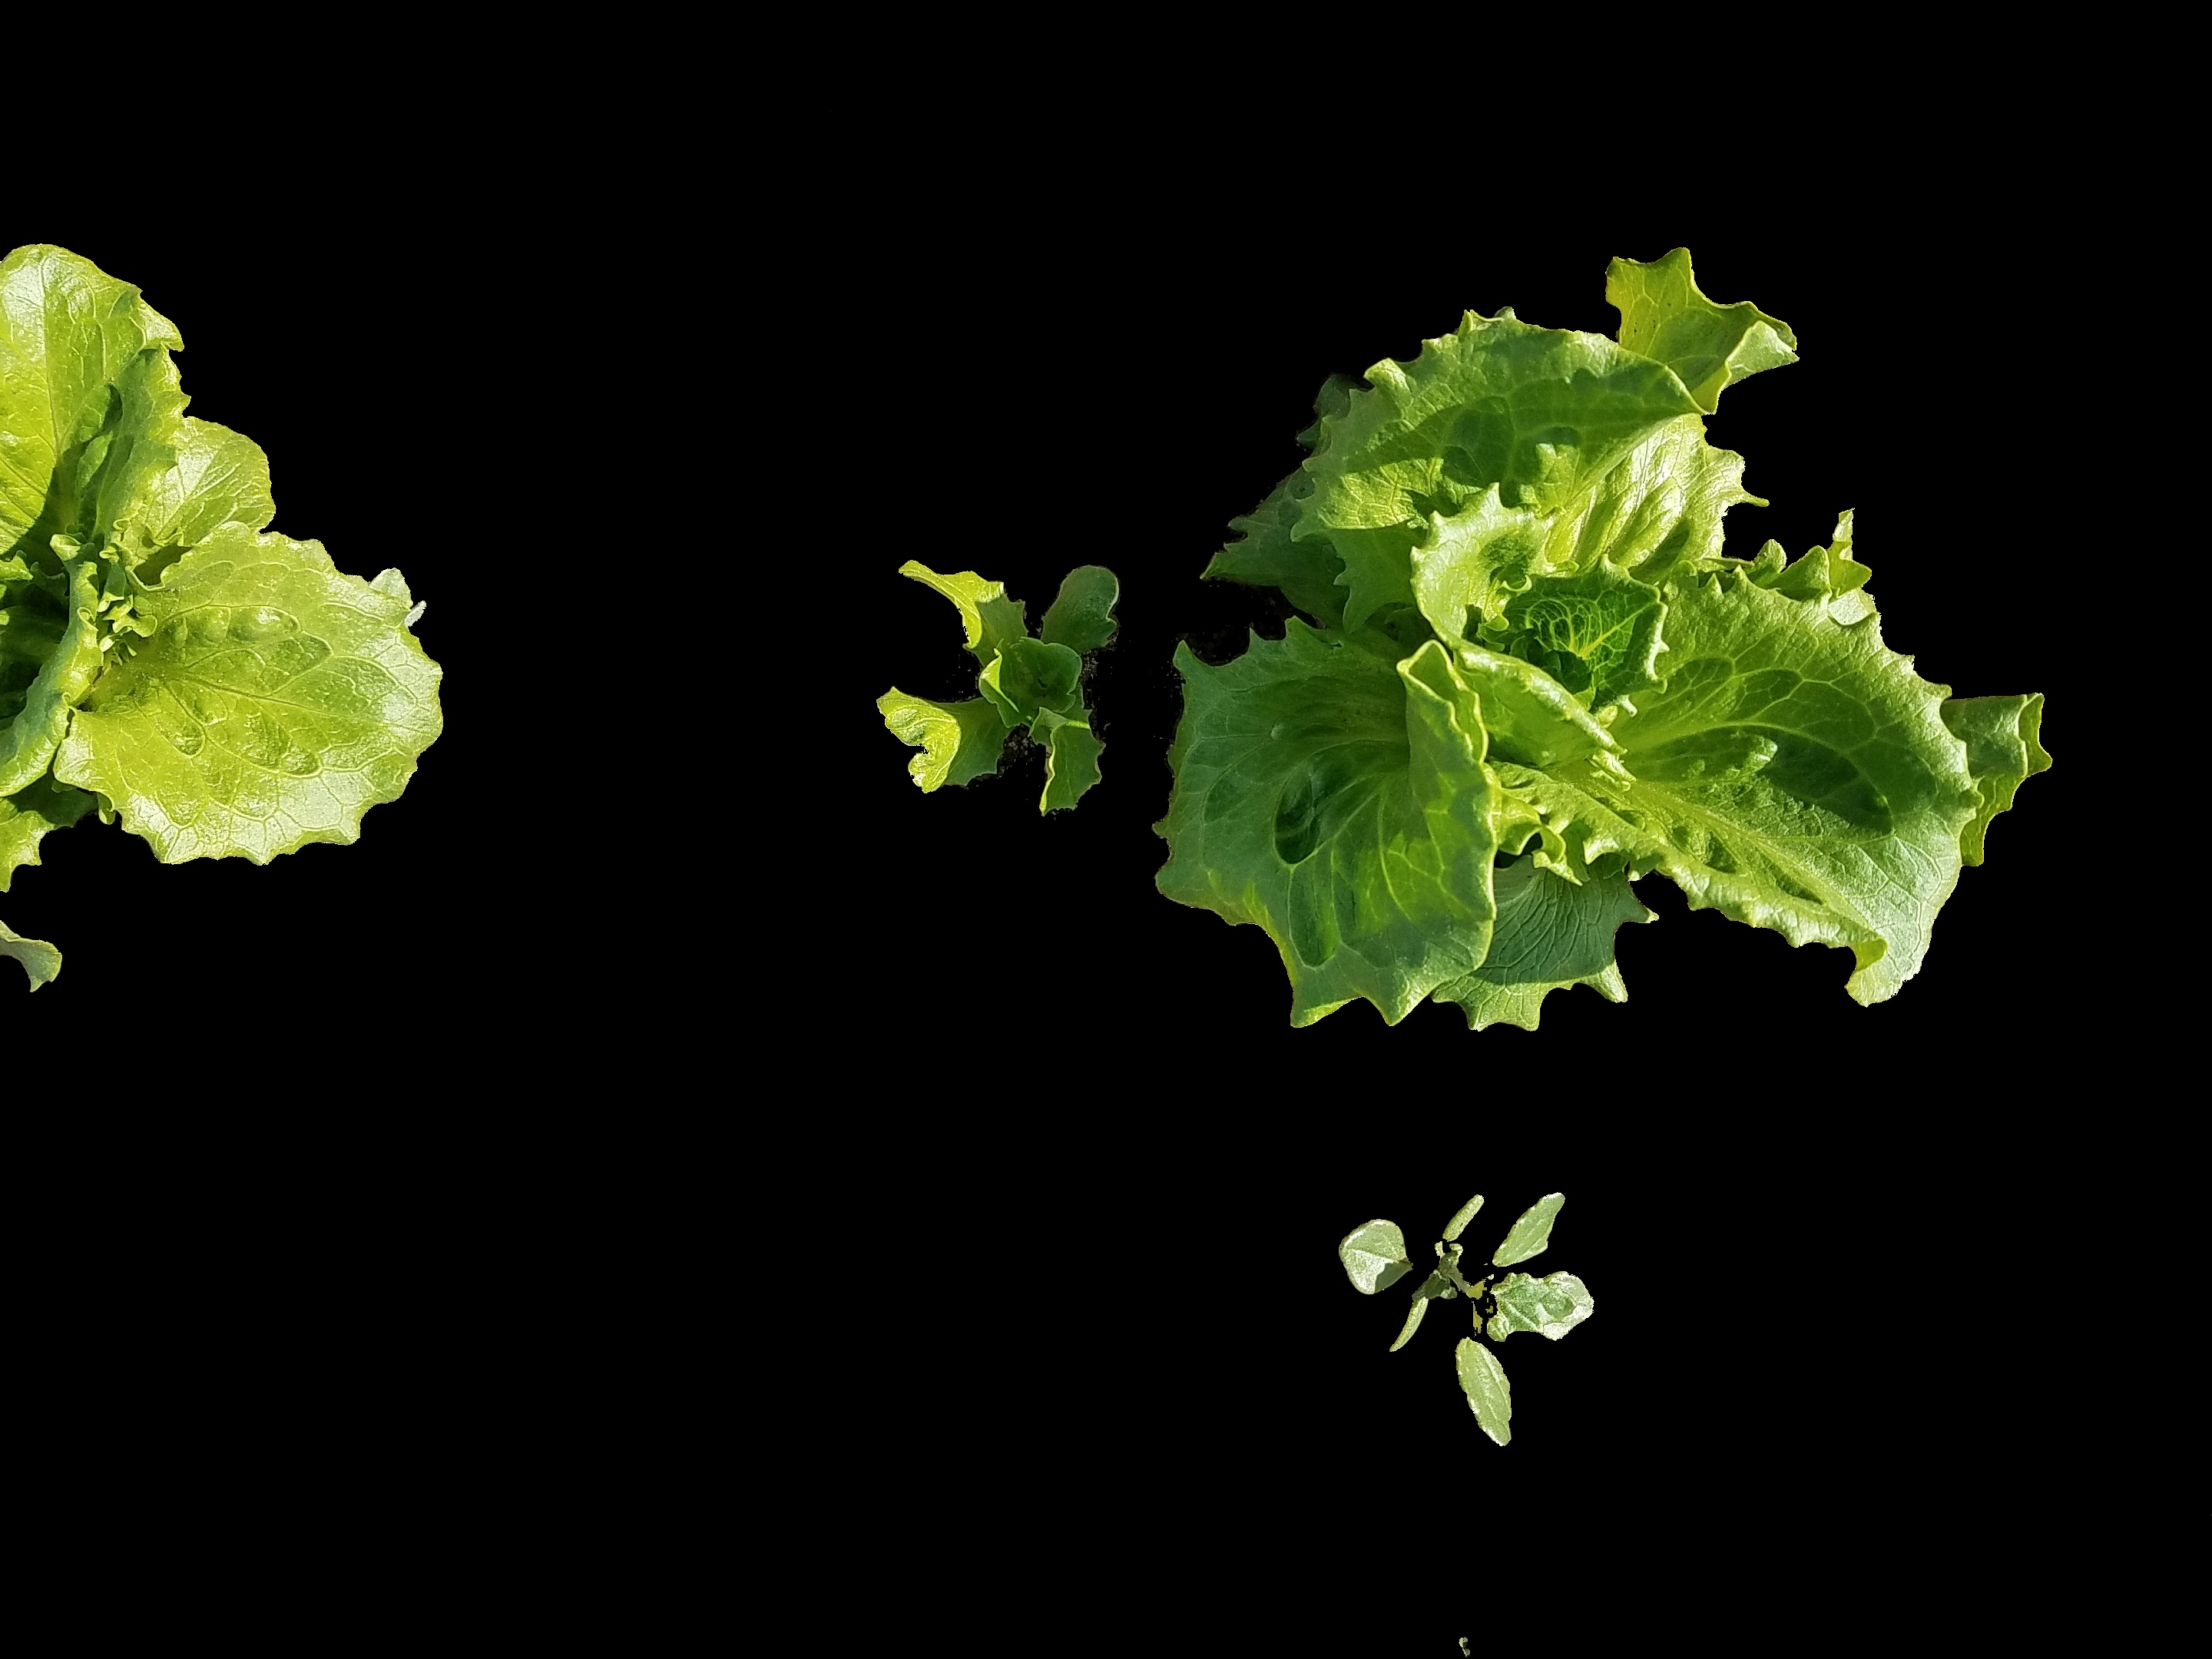
\includegraphics[width=1\linewidth]{figures/original-masked.jpg}
	  \caption{Mask applied}
	  \label{fig:original-masked}
	\end{subfigure}
	\caption[Before and after segmentation]{Before and after segmentation. The original image is used to produce the mask subsequently applied to produce the final image with only vegetated pixels remaining. Note the absence of the stems seen in the weed in the lower portion of~\ref{fig:original-masked} -- this is made a bit more obvious with a close examination of the mask shown in~\ref{fig:mask}. The lack of stems will lead to a single plant being identified as multiple plants, but has no effect on the classification using the features identified as significant. This is expected to be encountered more frequently in images taken from lower distances AGL, as individual pixels capture portions of vegetation that are not as green as other portions of the vegetation.}
	\label{fig:segmentation}
\end{figure}
%{\renewcommand{\arraystretch}{2}%
%
%{
%% This avoids the document line spacing affecting the contents of the table
%\setstretch{1.0}
%% Example to span two pages
%\begin{longtable}{x{\dimexpr.25\columnwidth-2\tabcolsep}
%                  x{\dimexpr.35\columnwidth-2\tabcolsep}
%                  x{\dimexpr.4\columnwidth-2\tabcolsep}}
%%\begin{hyphenrules}{nohyphenation}
%    \caption{Visible light indices}\label{tab:example}  \\
%\toprule
%{\textbf{Index}} & {\textbf{Formula}} & {\textbf{Comment}}
%\tabularnewline
%\midrule
%    \endfirsthead
%%%%%
%    \caption{Visible light indices (cont.)}\label{tab:example}  \\
%\toprule
%{\textbf{Index}} & {\textbf{Formula}} & {\textbf{Comment}}
%\tabularnewline
%\midrule
%    \endhead
%%%%%
%\midrule[\heavyrulewidth]
%\multicolumn{3}{r}{\footnotesize\itshape
%                   Continued on the next page}
%    \endfoot
%%%%%
%\bottomrule
%    \endlastfoot
%%%%%
%		Triangular Greenness
%		& \begin{minipage}[t]{0.3\textwidth}
%			$R_{green} - \alpha R_{red} - \beta R_{blue}\\ \alpha = \frac {2(\lambda_{blue} - \lambda_{green})} {(\lambda_{blue} - \lambda_{red})}\\ 
%		    	\beta = \frac {2(\lambda_{green} - \lambda_{red})} {(\lambda_{blue} - \lambda_{red})} $
%		   \end{minipage}     
%		& Corrects for camera calibration using the peak sensitivity
%\tabularnewline\addlinespace
%
%		Normalized Difference     
%		& $128 * \left( \left( \frac {(G - R)} {(G + R)} \right) + 1 \right) $                    
%		& The NDI index produces a near-binary image. 
%\tabularnewline\addlinespace
%
%		Excess Green      
%		& \begin{minipage}[t]{0.3\textwidth}
%			$R = \frac {R} {R_{max}}\\ G = \frac {G} {G_{max}}\\ B = \frac {B} {B_{max}}$ 
%		   \end{minipage}
%		& ExG provided a clear contrast between plants and soil 
%\tabularnewline\addlinespace
%
%		Excess Red      
%		& $1.3 R - G$ 
%		& inspired by the fact that there are 4\% blue, and 32\% green, compared with 64\% red cones in the retina of the human eye
%\tabularnewline\addlinespace
%
%		Color Index of Vegetation Extraction      
%		& $0.441 R - 0.811 G + 0.385 B + 18.78745$
%		& This method was proposed to separate green plants from soil background in order to evaluate the crop growing status.
%\tabularnewline\addlinespace
%
%		Excess Green - Excess Red   
%		& $ExG - ExR$ 
%		& ExG used to extract the plant region and ExR used to eliminate the background noise (soil and residue) where green–red material (stems, branches, or petioles) may exist
%\tabularnewline\addlinespace
%
%		Normalized Green-Red Difference    
%		& $\frac {(G - R)} {(G + R)}$ 
%		& The method of NGRDI was used to overcome the differences in exposure settings selected by the digital camera when acquiring aerial photography of the field. 
%\tabularnewline\addlinespace
%
%		Vegetative Index      
%		& $\frac {G} {R^aB^{(1-a)}}, a = 0.667$ 
%		& VEG has a significant advantage because it is robust to lighting change.
%\tabularnewline\addlinespace
%
%		Com1   
%		& $ExG + CIVE + ExGR + VEG$ 
%		& High computational cost --- does not perform well in high or low light levels
%\tabularnewline\addlinespace
%
%		Modified Excess Green      
%		& $1.262G - 0.884R = 0.311B$ 
%		& Does not perform well in high or low light levels. 
%\tabularnewline\addlinespace
%
%		Combined Indices 2      
%		& $0.36ExG + 0.47CIVE + 0.17VEG$ 
%		& Uses weighting factors to emphasize strengths of various approaches
%%\tabularnewline\addlinespace
%\label{table:segmentation}
%\end{longtable}
%}
Once the image contains only vegetated pixels, interrupted sections are presumed to be of the same plant.\footnote{This approach will not work well for situations where overlapping vegetation is frequently encountered (as would be expected for field crops) or where weeds and crop are in close proximity. This is the one of the primary motivations for focusing this study on crops where neither of these cases are commonly encountered, although proximal overlap of weeds and crop will certainly be encountered.} As contiguous regions of vegetated pixels are often referred to as \textit{blobs}, that is the term adopted within this document. A blob is simply an unclassified plant in this context, as processing the original image with an index has ensured that only vegetated pixels remain.



\subsection{Feature Extraction}
Identical sets of features are extracted from each feature set, regardless of altitude. The features of the vegetation considered here can be thought of as falling into three categories: color, structure, and texture.  Features represent only a single value for a blob, i.e., the mean value of the blob's hue is 0.7443 or the roundness of a blob is 0.5302.
\subsubsection{Color}
Color features involve the expression of the familiar Red, Green, and Blue wavelengths typically considered when discussing images, but also includes colorspaces less commonly discussed: Hue, Saturation, and Intensity (HSI); Hue, Saturation, and Value (HSV); YIQ; YCBCR; and CIElab. In each of these spaces, various expressions (mean, standard deviation) of a blob's channels will be treated as a feature. The standard deviation of the \textit{in-phase} values of a blob in the YIQ space, for instance, would be considered as an extracted feature.
\subsubsection{Structure}
Structural Features involve both expressions of a blob's shape (how close it is to being circular, for example) and a blob's surface (a leaf's surface, can be thought of as having quantifiable \textit{texture}).  Shape factors that will be computed include: an object's convex hull, elongation, perimeter, eccentricity, convexity, compactness, circularity, and shape index. (\cite{Lin2017-xq, Wirth2004-li}) Surface features can be expressed with textural metrics such as Grey Level Co-occurrence Matrix (GLCM) \parencite{Haralick1973-gr, Hall-Beyer2017-nx} While images are converted to greyscale to achieve the metrics \citeauthor{Haralick1973-gr} detail, the GLCM expressions will also be computed for each of the aforementioned color spaces. For instance, the expression of the \textit{energy} of the blob's \textit{hue} in the HSI colorspace is an example of a co-occurrence calculation used to describe the blob. The blob can also be described its gradients. Extracting information about these gradient using the Histogram of Oriented Gradients (HOG) and subsequently using that information in manipulations yields a descriptor for that blob.\parencite{Abouzahir2021-sd}. As outlined in \ref{sec:acquisition}, images will be acquired at different altitudes, and it is likely the case that the most significant features relevant for classification will not remain constant with increasing altitude. Shape metrics, for example, may be less significant at 10m than at 2m, given that fine edge details are not present in images taken from higher distances AGL.


\subsection{Optimal Features}
Using the aforementioned features, each blob has approximately 715 features to describe it. To find which of these features are significant to the classification technique several statistical technique will be employed to produce the top 10 most influential parameters: PCA, Recursive Elimination, Feature Importance, and Univariate Feature Selection. Choosing the top 10 most influential parameters is itself excessive, as PCA shows that only a few parameters are responsible for most of the variance seen. While the initial stages of the classification will use the top 10 features, analysis of even smaller sets will be done as well.
\begin{figure}[h]
	%\centering
	\begin{subfigure}[h]{.48\textwidth}
		  \centering
		  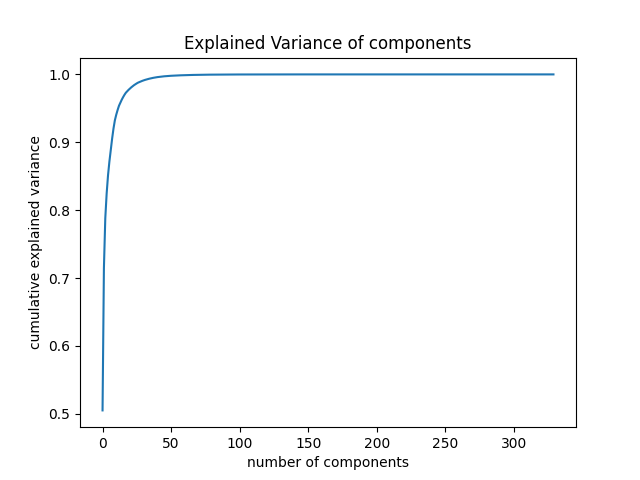
\includegraphics[width=1\linewidth]{figures/pca.png}
		  \caption{Features explaining variance}
		  \label{fig:pca}
	\end{subfigure}
	\begin{subfigure}[h]{.32\textwidth}
	  \centering
	  	
		{
		\centering\settowidth\rotheadsize{\bfseries(our proposal)}
		\renewcommand\theadalign{cl}\renewcommand\cellalign{cl}
		\renewcommand\theadfont{\bfseries}
		\renewcommand\tabcolsep{4pt}\renewcommand\arraystretch{1.25}
		% Make this a bit smaller so it will fit on a page.  Still looks a bit nasty in that it extends to the edge of the page.
		% It's that PCA line that is the trouble, as the values are just too long
		\footnotesize
		
		\begin{longtable}[c]{
		    |l |*{12}{c |} }%
		    \hline
		    %\diagbox[height=1.2\rotheadsize, width=\dimexpr\eqboxwidth{AB}+2\tabcolsep\relax]%
		    %{\raisebox{1.2ex}{Feature}}{\raisebox{-5ex}{Feature}} &
		    {\textbf{Feature}} & {\textbf{Importance Rank}}\\
		    %\rothead{Tool X\\\mbox{(our proposal)}}\\
		    \hline
			hue                      &     0.505089 \\
			saturation\_mean          &     0.209646 \\
			in\_phase                 &     0.073444 \\
			cb\_mean                  &     0.036392 \\
			hog\_stddev               &     0.026874 \\
			hog\_mean                 &     0.020135 \\
			hog\_variance             &     0.017359 \\
			greyscale\_homogeneity\_0  &     0.016602 \\
			greyscale\_homogeneity\_45 &     0.014872 \\
			greyscale\_homogeneity\_90 &     0.012052 \\	    
		    
		    \hline
		    %\caption{Feature Importance Ranks using RFE with a Random Forest Classifier}
		    %\label{fig:random-forest}
		  \end{longtable}
		 }
	  \caption{PCA Variances}
  %\label{fig:sub2}
	\end{subfigure}
\caption{Principal Component Analysis of Features}
\label{fig:pca}
\end{figure}


Early work has shown that these four techniques yield a list of 36 unique parameters, and that use of the parameter set produced by one approach will yield poor results with one particular model, but excellent results with another. To arrive at the optimal set for each model, all combinations of the 36 parameters taken 10 at a time will be evaluated.\footnote{The combination of 36 parameters taken 10 at a time is a reasonably large number, 254,185,856.  As we are evaluating seven different  machine learning techniques, this yields 1,779,307,992 models that will be built and evaluated. As my home machine can build only 1.5 million models overnight, the university HPCC is more suitable for this phase. As evaluating that number of models requires several days of computation, it may be the case that feature selection techniques (and thus the search space) is reduced.} That is, a model will be built for each combination of unique parameters to determine the best set for each technique at each altitude.
In this use case, \textit{Evaluated} is somewhat more complex than it first appears. While overall accuracy is certainly important, these models will be evaluated in terms of maximizing the true positive rate of the classification of weeds as weeds while minimizing the false positive rate of classifying crop as weeds. Evaluating the model using the Area Under the Curve (AUC) and Receiver Operating Characteristic (ROC) curves is insightful, but these approaches are not sensitive to the fact that a mistaken classification of weed as crop has a much lower impact than the mistaken classification of a crop as a weed.\\


\subsection{Labeling}
The proposed study will use a supervised approach, one that depends on a labeled data set. That is, a human expert must determine if a plant is a weed or a crop. In support of this manual process, a user will employ a custom application to step through the images and identify the class of vegetation. Commercial  applications (such as LabelBox) are convenient, of course, but do not fit in well with the workflow presented here, focused on DB integration.

\subsection{Classification}
The set of optimal parameters will be used for binary classification using various ML classification techniques: Random Forest, Linear Discriminant Analysis (LDA), Support Vector Machine (SVM), Decision Tree, Logistic Regression, and Gradient Boosting.\footnote{These techniques are the ones currently coded, but the cost of the addition of other techniques is fairly low (the addition of LDA, for instance, was fairly recent and was integrated into the existing within a few minutes). Incorporating a deep learning approach has a somewhat higher, but not overly disruptive cost. This list of techniques can be expanded without significant change to other workflow steps described.} The raw images gathered in the field will be annotated with these classifications and subsequently manually inspected and corrected.\\
As more images are acquired across the data development cycle, the manually corrected training data set will grow larger and is expected to contain both crop and weed images at various stages of development. This holds true for crop in particular, as remediation will likely remove them from the image sets before they are fully developed. This dataset will then be used to classify vegetation in a subsequent development cycle. While the subsequent development cycle image acquisition will follow the same procedures, it is anticipated that the correct classification of weeds will not only be higher, but that the resulting training set can be generalized across the development cycle. That is, any point in second development cycle can use the training set from the first.
\begin{figure}[h]
	\centering
	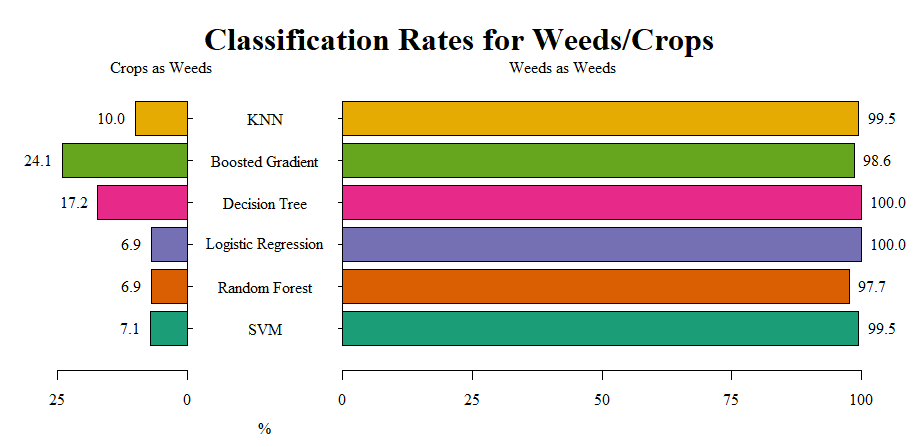
\includegraphics[width=0.7\linewidth]{./figures/classification-rates.png}
	\caption[Misclassification rates of various algorithms for sample images]{The correct and misclassification rates of various algorithms using a sample image set are shown here. While an overall accuracy of 95.7\% may sound impressive for the Boosted Gradient algorithm, considering the salient misclassification and correct classification rates, 24.1\% and 98.6\%, respectively, that algorithm does not support the accuracy needed in this use case, as the cost of the misclassification of crops as weeds is quite high.}
	\label{fig:classification-rates}
\end{figure}

\subsection{Implementation Details}
This phase of the project involves three compute platforms:
\begin{itemize}
	\item{Classification analysis will be done in R on a general-purpose desktop computer or laptop. No special equipment or software is required for this other than the use of R/R Studio itself.}
	\item{Feature analysis will be done on the University of Arizona's High-Performance Compute Cluster (HPCC), using software written in Python. The software will use ML libraries provided by the scikit-learn offering, but has no other dependencies otherwise.}
	\item{Images collected in the field will be segmented and classified on a single-board (SBC) running Linux (Seeed Studio Odyssey). While the details of this deployment will be provided in a separate document, this will involve: Docker, MongoDB, Python3, and scikit-learn.}
\end{itemize}
All the software for each of these platforms can be accessed through a GitHub repository. Making the data acquired and subsequently classified as part of this project available has not yet been finalized. All data (raw images, for instance) is kept in a database and easily exported, but no  firm plans are in place to expose the raw or processed images or to expose the database itself.

\section{Phase II}
This phase concentrates on the production of a treatment plan from the classification results. The treatment plan is intended for human consumption, noting the details that include the location (geographic and row/offset position) of each plant. While the implementation and analysis of an automated treatment system is beyond the scope of this study, this phase will demonstrate a workflow similar to what an automate system would employ.
As there could be many hundreds of weeds within a single field, it is not likely that a report detailing the particulars of each weed would prove to be an effective mechanism. A treatment plan will instead be more of an exploratory tool for the data, allowing the user to drill down into data from the field level to an individual plant. To facilitate this sort of interaction, the simplified model shown in Figure \ref{fig:architecture} will be used. Here, the user explores the data via a tablet application, which, in turn, retrieves information through the back-end weed server and database\footnote{Implementation details are beyond the scope of this document, but it is reasonable to see this as a fairly standard three-tier deployment, with clean separation between user interface (the exploration application), business logic (the weed server), and data. The weed server exposes an API and is unaware of the details of exactly how this information will be used. Likewise, the application is unaware of how the information is stored or processed. While it may be the case that the server is realized as a Flask application and the data resides in a MongoDB, these are implementation details that have no impact on other application tiers.} Information in this database is populated by the classifier discussed in Phase I. The deployment of these components is fairly flexible.  While the user and tablet are in the field or office, other components can reside either within a hosted (i.e., cloud) or resident deployment. The deliverable in this phase is the tablet-based application through which the user views information about the crop and weeds.\footnote{While a phone-based application is possible, and is certainly not precluded from this architecture (indeed it would be a component that could coexist beside the tablet application), a phone application is not part of this proposal}
\begin{figure}[h]
	\centering
	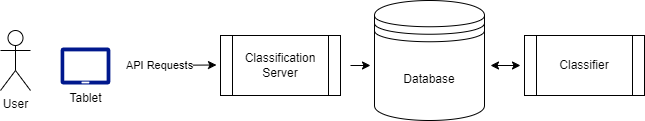
\includegraphics[width=0.8\linewidth]{./figures/treatment-plan-explore.drawio.png}
	\caption[Exploration of the classified dataset]{The user and tablet are typically present in the field or office, exploring the data, while the server, database, and classifier are present in the field or a hosted environment. The classification server accepts API requests from the tablet application, allowing the user to explore the treatment sets without tightly coupling the two. In this scenario, previously collected data, effectively making it an off-line solution.}
	\label{fig:architecture}
\end{figure}

The tablet application will be realized using Python 3.8/PyQt5 and deployed on Microsoft Surface hardware. While Surface tablet will be used for deployment, a Windows 10 desktop can also be used. as that is where development will take place.

The exploration of the classified data highlights a relatively glaring omission: the precise location of vegetation. While the images collected by the UAV are tagged with the latitude and longitude of the observation, the accuracy of the coordinates is not within the range suitable for a subsequent precision treatment. While a pixel offset of the weed's center within the image can be very precise (a basic geometric problem), the location of the image may be off by several centimeters, resulting in a location that is useful for casual exploration of the data, but not for precision treatment.  The UAV specified in the phase I uses an uncorrected GPS\footnote{descriptions of corrections via RTK or PPK are beyond the scope of this document, but are typically employed to achieve the sub-centimeter accuracy required)}. While the location of the vegetation can given as an inaccurate position or a relatively accurate relative position (row 3, 32.25 meters from the start of the row), neither of these are suitable for precision treatment. The use of corrected GPS would not require changes to the workflow proposed, but will not be employed in this study.
 
This deployment is not limited to human interaction, of course. If the human interaction were replaced by an automated remediation, the overall deployment is completely unchanged, as Figure \ref{fig:architecture-with-treatment} illustrates.
\begin{figure}[h]
	\centering
	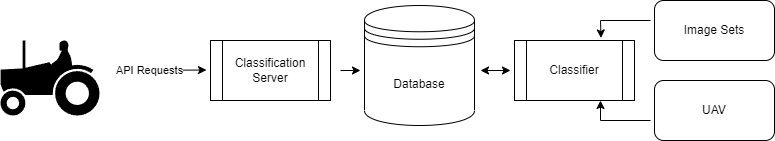
\includegraphics[width=0.8\linewidth]{./figures/treatment-plan.drawio.png}
	\caption[Simplified View of System Architecture]{If instead of exploring the data the focus is on the application of treatment -- as would be the case with a towed sprayer or drone system, the overall architecture is unchanged. In this deployment, nothing has changed with the server deployment, as it continues to service requests. In this more real-time solution, images are classified immediately after acquisition. It should be noted, however, that development of a real-time classification and treatment system is not within the scope of this project, only that this system lends itself to this deployment. While this figure illustrates the use of a towed solution, where components can be deployed on a small form factor PC, the solution can also be deployed on board a UAV's co-processing system. Some UAVs offered by DJI support such a co-processor, but integration that solution is a Phase III, beyond the scope of this work.}
	\label{fig:architecture-with-treatment}
\end{figure}
%\subsection{Weed Geolocation}
%For both the automated treatment and human exploration of treatment plans, accuracy of 1cm is desired.  That is, the location of a weed is not limited by a (row, edge-offset) location scheme, or a smartphone-level accuracy of 5m or so. Rather, the location of vegetation lend itself to precision treatment.
%While image sets are augmented with high-precision geo-location data, this phase will also compare the ground-truth location data of weeds to the projected location recorded by drone.\footnote{Image sets that are manually acquired (hand-held phone pictures) will not include high-precision location data, and are not considered as part of this step} Aside from best practices such as a clear view of the sky or using a high-quality antenna, GPS location data can be improved by applying correction data. This will involve two new pieces of equipment: a Real Time Kinematics (RTK) base station transmitting corrections, and a rover (manually moved survey pole) within the field capable of using those corrections.\footnote{It is not the case that a low-accuracy GPS such as would be found in a phone would be suddenly improved with this data. Rather, the GPS must be capable of applying the corrections. I have such a base station on my roof and a rover on my desk. While off-the-shelf solutions are available, these can be built fairly inexpensively} The RTK base station will reside with 10km of the field location if correction is provided over an internet connection and within 300m if corrections are provided over a radio link. In either deployment scenario, the field personnel positions a GPS equipped survey pole, referred to as a \textit{rover}, in close proximity to the plant to record the location of each.\footnote{It remains to be seen if recording the location of the weed is a manual process or one where a user simply presses a button on a tablet application to record the location. Given my distrust of any manual process, it will likely be the latter, although that means more software to write. It is also not required that the plant in question are weeds, or are classified as such. The purpose of this step is to assess the positional difference between locations extracted from UAV images and that determined from a separate ground system.}
%\begin{figure}[h]
%	\centering
%	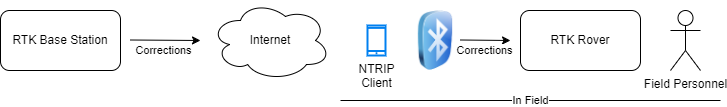
\includegraphics[width=0.8\linewidth]{./figures/rtk-internet.drawio.png}
%	\caption[RTK corrections delivered through Internet]{RTK corrections can be delivered through the Internet to a RTK-capable GPS receiver in the field if an Internet connected, bluetooth enabled cellphone with an NTRIP client is present near the GPS. The NTRIP client serves as a sort of bridge between corrections obtained from the Internet and the GPS. This deployment has a limitation that there can be at most 10km between the base station and rover.}
%	\label{fig:rtk-internet}
%\end{figure}
%\begin{figure}[h]
%	\centering
%	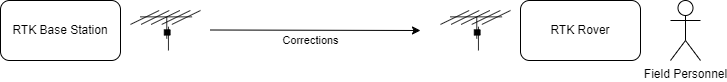
\includegraphics[width=0.8\linewidth]{./figures/rtk-radio.drawio.png}
%	\caption[RTK corrections delivered via Radio]{For locations with limited Internet connectivity, corrections are delivered directly to the RTK-capable GPS via a radio link. This deployment has a limitation that there can be at most 300m between the rover and base station with a clear line of sight between the two.}
%	\label{fig:rtk-radio}
%\end{figure}
%
%Irrespective of the location technique employed, a sample of vegetation location will be taken to ensure a 95\% confidence interval with a 5\% margin of error.

\subsection{Timeline of Activities}
Image acquisition will commence four weeks after planting and will take place every two weeks until harvest.\footnote{Capturing images every two weeks may be overkill, and may changes to a longer interval if no significant change is seen between captures. This should be considered as a worst-case schedule.} As the planting date has not been fixed at the time of this writing (but has tentatively targeted for the first half of December 2023), the schedule will follow a T0 (planting) plus timing. An overview\footnote{The full agile board containing details beyond this list comprising the entire backlog is also available -- contact the author for access to: \href{https://evan-mcginnis.atlassian.net/jira/software/c/projects/WEED/boards/1}{Agile-Board}} of the activities and milestones is summarized by Table~\ref{tab:timeline}. As the study timeline and the academic timeline are inextricably linked, both are presented here, but as dates for the latter have not yet been scheduled, they are tentative and will be updated as needed.
\begin{table}[ht]
	\centering
    \caption{Study timeline in elapsed weeks}
    \label{tab:timeline}
    \begin{tabular}[t]{lll} 
		\textbf{T0+} & \textbf{Activity} &\textbf{Comments}\\
		\midrule
			4 & Image Collection & At MAC\\
			6 & Image Collection & At MAC\\
			8 & Image Collection & At MAC\\
			10 & Image Collection & At MAC\\
			12 & Image Collection & At MAC\\
			14 & Image Collection & At MAC\\
			16 & Image Collection & At MAC\\
			17 & \textit{Initial Findings Ready} & \\
			18 & Image Collection & At MAC\\
			20 & Image Collection (If needed) & At MAC \\
			22 & Image Collection (If needed) & At MAC \\
			30 & Paper on classification ready for internal review & \\
			36 & \textit{Phase II Treatment Map Ready} & \\
			40 & Paper on color differences ready for internal review & \\
    \end{tabular}
\end{table}

Of particular interest here is the time of initial findings. The initial findings will include items discussed in previous sections of this document: optimal features at each altitude for each technique. The images gathered from subsequent collections are not expected to materially change those findings, but those initial findings will be updated to incorporate data extracted from those image sets. The paper describing the classification of vegetation will be ready for internal review by the 30$^{th}$ week. This paper will not cover details of segmentation or implementation, but will present a fairly complete picture of Phase I results. The second paper is, unfortunately, less well defined, as the content will depend greatly on the problems encountered and characteristics of the crop. Two topics stand out from early work: prediction with the imbalanced data set found in the fields (e.g., there are much more crop plants than weeds in some plantings, as will be expected in the drip-irrigated spinach field in this study), and color differences between irrigation techniques (i.e., drip and center-pivot colors may vary).

\begin{table}[ht]
	\centering
    \caption{Academic timeline}
    \label{tab:timeline}
    \begin{tabular}[t]{lll} 
		\textbf{Date} & \textbf{Activity} &\textbf{Comments}\\
		\midrule
			December 2023 & Written Comprehensive & Not yet scheduled\\
			February 2024 & Oral Comprehensive & Not yet scheduled\\
			March 2025 & Thesis available for review & Tentative\\
			April 2025 & Defense & Not yet scheduled\\

    \end{tabular}
\end{table}

 \newpage
%
% W E A K N E S S E S
%
%\section{Weaknesses of Proposal}
%This proposal has weaknesses in how the findings can be generalized to other row crops or locations where the weed population may differ. As the targeted crop is fixed, it may be the case that factors that are indicative of one crop (lettuce, for instance) hold the same significance for another (cotton, for instance). Likewise, the weed population encountered in one area may not be present in another. 

\newpage
\section{Appendix A -- Implementation}
\subsection{Development Environment}
Software will be written in Python 3 and R in this environment:

\begin{itemize}
	\item{OS: Windows 10}
	\item{IDE: PyCharm 2022.3, RStudio 2023.03.0+386}
	\item{Language: Python 3.8, R}
	\item{Image Processing: OpenCV, Scikit-image}
	\item{Machine Learning: Scikit Learn}
	\item{UI Development: PyQt5}
\end{itemize}

While various Python and R libraries not noted will also be used, this set forms the core of what will be used.

\subsection{Deployment Environment}
While the software developed is not tightly coupled to a specific OS, the deployment environment will consist of:
\begin{itemize}
	\item{Linux kernel 5.4 (Ubuntu distribution)}
	\item{Docker 24.0.2}
	\item{MongoDB 4.4.5 Community Edition}
	\item{NGINX 1.24.0}
\end{itemize}

While an Ubuntu distribution is shown in the list above, deploying the solution to Windows or Centos does not require substantial changes. This flexibility is what will allow the migration of the software from a deployment in the author's office to one where the AUV hosts all software.  Some DJI models, for example, allow the addition of a GPU or CPU based system nearly identical to the one used in testing.








\newpage
{
\setstretch{1.0}
\section{References}
\printbibliography[heading=none]
}

\end{document}

